\section{Methods}
\label{sec:methods}

We approached EK-100 MIR as an iterative search through the design space, starting from a feature-based zero-fine-tuning baseline and ending with end-to-end fine-tuning of a strong egocentric backbone with soft-label supervision. The three approaches share a common formalisation, stated once before each iteration is described.

\subsection{Task formalisation and common notation}
\label{sec:methods:formalisation}

Let $\mathcal{V} = \{v_i\}_{i=1}^{N_v}$ denote the $N_v = 9{,}668$ test video segments and $\mathcal{T} = \{t_j\}_{j=1}^{N_t}$ the $N_t = 3{,}842$ unique text queries on the test split. A retrieval system produces a similarity matrix $S \in \mathbb{R}^{N_v\times N_t}$ such that $S_{ij}$ is large when $v_i$ is semantically relevant to $t_j$. Ground-truth relevance is encoded in the soft-label matrix $R \in [0,1]^{N_v\times N_t}$~\cite{wray2021semantic}; the official challenge metric is the average normalised discounted cumulative gain
\begin{equation}
\mathrm{nDCG}_{\mathrm{AVG}} = \tfrac{1}{2}\bigl(\mathrm{nDCG}_{\mathrm{V\to T}}(S, R) + \mathrm{nDCG}_{\mathrm{T\to V}}(S^{\!\top}\!, R^{\!\top})\bigr),
\label{eq:ndcg}
\end{equation}
which captures both retrieval directions on equal footing. The three approaches differ only in how $S$ is constructed; the evaluation protocol is identical across them. Figure~\ref{fig:solutionflow} summarises the resulting pipeline.

\begin{figure}[t]
    \centering
    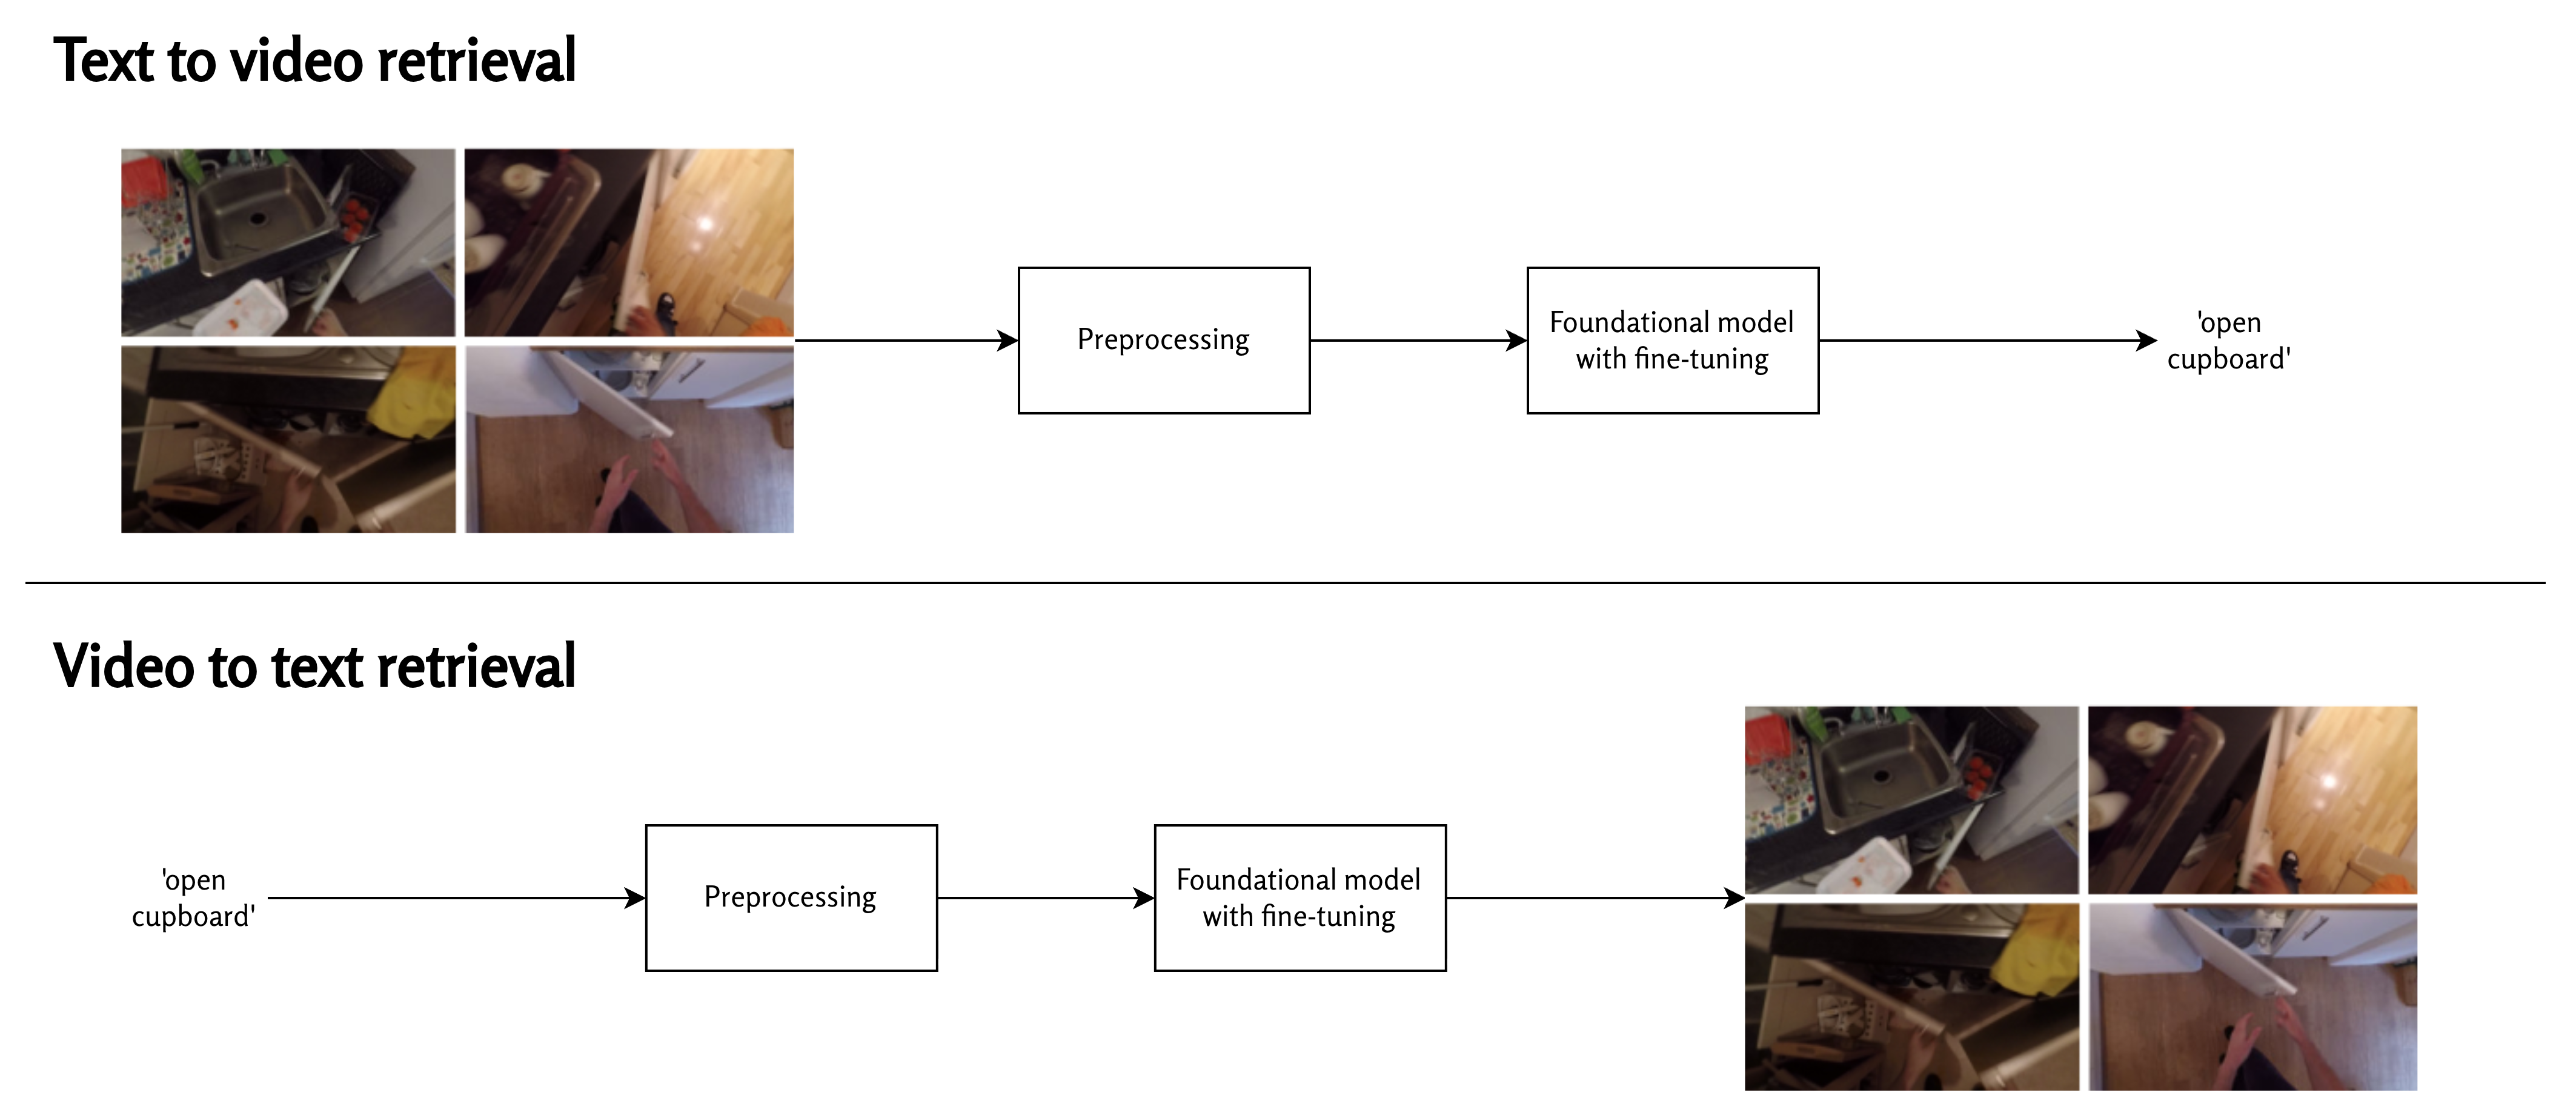
\includegraphics[width=0.7\textwidth]{images/flow.png}
    \caption{Overview of the multi-instance retrieval pipeline shared by the three approaches: visual and textual encoders project segments and queries into a shared space, and the resulting similarity matrix $S$ is ranked and evaluated against the soft-label matrix $R$. Image components adapted from~\cite{damen2022rescaling}.}
    \label{fig:solutionflow}
\end{figure}

\subsection{Approach 1: JPoSE Part-of-Speech baseline}
\label{sec:methods:jpose}

Our entry point is a feature-based, zero-fine-tuning baseline using JPoSE~\cite{wray2019jpose}, which projects segments and queries into three sub-spaces---verb, noun and full-action---learnt jointly with triplet supervision. Let $\phi^{\mathrm{v}}_{\mathrm{V}}, \phi^{\mathrm{v}}_{\mathrm{N}}, \phi^{\mathrm{v}}_{\mathrm{A}}$ and $\phi^{\mathrm{t}}_{\mathrm{V}}, \phi^{\mathrm{t}}_{\mathrm{N}}, \phi^{\mathrm{t}}_{\mathrm{A}}$ denote the visual and textual sub-encoders. We compute joint embeddings as the concatenation $\mathbf{f}_{\mathrm{v}}(v_i) = [\phi^{\mathrm{v}}_{\mathrm{V}}(v_i)\,;\,\phi^{\mathrm{v}}_{\mathrm{N}}(v_i)\,;\,\phi^{\mathrm{v}}_{\mathrm{A}}(v_i)]$ and analogously $\mathbf{f}_{\mathrm{t}}(t_j)$, and obtain $S^{\mathrm{JPoSE}}_{ij} = \cos(\mathbf{f}_{\mathrm{v}}(v_i), \mathbf{f}_{\mathrm{t}}(t_j))$. We use the released \texttt{JPoSE\_BEST} checkpoint without modification on pre-extracted features. By design this approach cannot exploit $R$ and inherits the limitations of triplet supervision with binary positives and negatives, but it provides a reproducible reference point against which all subsequent iterations are compared.

\subsection{Approach 2: score-level ensemble with graph-diffusion re-ranking}
\label{sec:methods:ensemble}

The second approach asks how far a purely inference-time strategy can carry the JPoSE baseline by combining several pre-trained retrieval models and refining the result with neighbourhood-aware re-ranking. Three complementary models are queried independently: $S^{\mathrm{JPoSE}}$ as in Section~\ref{sec:methods:jpose}; $S^{\mathrm{MI\text{-}MM}}$, the multi-instance MaxMargin model of Miech et al.~\cite{miech2020milnce} with S3D-HowTo100M features at the released best epoch (202); and $S^{\mathrm{MMEN}}$, an MLP-based Multi-Modal Embedding Network released as a baseline in~\cite{wray2019jpose}.

\paragraph{Step 1: row-wise normalisation and equal-weight fusion.}
The three matrices live on different scales (cosine similarities for JPoSE/MMEN, max-margin distances for MI-MM), so a direct sum is biased towards the highest-magnitude model. We min-max normalise each matrix \emph{row-wise} so that, for every video query, scores against the $3{,}842$ candidates are mapped to $[0,1]$:
\begin{equation}
\widetilde{S}^{(m)}_{ij} = \frac{S^{(m)}_{ij} - \min_k S^{(m)}_{ik}}{\max_k S^{(m)}_{ik} - \min_k S^{(m)}_{ik}}\,,\quad
S^{\mathrm{ens}} = \tfrac{1}{3}\,(\widetilde{S}^{\mathrm{JPoSE}} + \widetilde{S}^{\mathrm{MI\text{-}MM}} + \widetilde{S}^{\mathrm{MMEN}}).
\label{eq:ensemble}
\end{equation}
Equal weights are the natural default in the absence of a relevance-aligned validation signal.

\paragraph{Step 2: graph-diffusion re-ranking on visual and textual k-NN graphs.}
Inspired by diffusion-based re-ranking in image retrieval~\cite{iscen2017diffusion} and k-reciprocal encoding~\cite{zhong2017kreciprocal}, we propagate ensemble scores through the local geometry of the retrieval space in both modalities. After L2-normalising each row of $S^{\mathrm{ens}}$, a sparse visual affinity matrix $A_{\mathrm{vv}} \in \mathbb{R}^{N_v\times N_v}$ stores cosine similarity between the score profiles of each pair of segments if either is among the top-$k$ visual neighbours of the other; the same construction on $(S^{\mathrm{ens}})^{\!\top}$ yields a textual affinity $A_{\mathrm{tt}}$. We then expand the score matrix in both directions and blend with the original ensemble:
\begin{equation}
S^{\mathrm{exp}} = \tfrac{1}{2}\,(A_{\mathrm{vv}}\,S^{\mathrm{ens}} + (A_{\mathrm{tt}}\,(S^{\mathrm{ens}})^{\!\top})^{\!\top}),\quad
S^{\mathrm{rerank}} = (1-\alpha)\,S^{\mathrm{ens}} + \alpha\,S^{\mathrm{exp}},
\label{eq:rerank}
\end{equation}
with default $k=20$, $\alpha=0.3$. Both the ensemble matrix~\eqref{eq:ensemble} and the re-ranked matrix~\eqref{eq:rerank} are submitted to Codabench as separate iterations, isolating the contribution of re-ranking.

\subsection{Approach 3: AVION ViT-L fine-tuned with the SMS loss}
\label{sec:methods:avion}

The third approach replaces inference-time fusion with end-to-end fine-tuning of a strong CLIP-style egocentric backbone, supervised with the soft-label relevance matrix. The visual encoder is the AVION ViT-L/14 of Zhao and Kr\"ahenb\"uhl~\cite{zhao2023avion}, pre-trained on Ego4D via LaViLa~\cite{zhao2023lavila}; the textual encoder is the CLIP text transformer paired with that AVION checkpoint. Both encoders are fine-tuned jointly with the Symmetric Multi-Similarity loss of Wang, Wang and Chau~\cite{wang2024symmetricmultisimilaritylossepickitchens100}.

\paragraph{Symmetric Multi-Similarity loss.}
Within a training batch of $B$ video--text pairs, let $\mathbf{x}_i, \mathbf{y}_i \in \mathbb{R}^d$ denote the L2-normalised visual and textual embeddings of pair $i$, $r_{ij} \in [0,1]$ the soft relevance between $v_i$ and $t_j$ extracted from $R$~\cite{wray2021semantic}, and $s_{ij} = \mathbf{x}_i^{\!\top}\mathbf{y}_j$. The SMS loss extends the multi-similarity formulation of~\cite{wang2019multisimilarity} so that, instead of binary pair weights, the contribution of each pair is modulated by $r_{ij}$. With margin $\theta$, relevance threshold $\tau$ and temperatures $\beta_p, \beta_n$,
\begin{equation}
\mathcal{L}^{\mathrm{V\to T}}_i = \tfrac{1}{\beta_p}\log\!\Bigl(1 + \!\!\sum_{j: r_{ij}\ge \tau}\!\! r_{ij}\,e^{-\beta_p(s_{ij}-\theta)}\Bigr) + \tfrac{1}{\beta_n}\log\!\Bigl(1 + \!\!\sum_{j: r_{ij}<\tau}\!\! (1-r_{ij})\,e^{\beta_n(s_{ij}-\theta)}\Bigr),
\label{eq:sms}
\end{equation}
and the full loss is the symmetric counterpart $\mathcal{L} = \tfrac{1}{2}(\mathcal{L}^{\mathrm{V\to T}} + \mathcal{L}^{\mathrm{T\to V}})$ averaged over the batch. Compared with InfoNCE-like contrastive losses, SMS pulls together pairs in proportion to their relevance and pushes apart pairs in proportion to $1 - r_{ij}$, providing a supervision signal directly aligned with the nDCG metric.

\paragraph{Fine-tuning configuration.}
Fine-tuning is launched from the AVION pretrain checkpoint via \texttt{ammplus\_finetune.py} from a patched fork of the public SMS-Loss codebase~\cite{wang2024smsloss_repo} on a single A100. Key flags: \texttt{--model CLIP\_VITL14}, \texttt{--batch-size 48}, \texttt{--lr 2e-5}, \texttt{--loss-margin 0.6}, \texttt{--loss-thres 0.1}, with \texttt{--use-fast-conv1}, \texttt{--grad-checkpointing} (essential for ViT-L on a single GPU) and \texttt{--use-flash-attn} when available; FlashAttention~\cite{dao2022flashattention} roughly halves attention memory at no accuracy cost. Optimisation uses AdamW~\cite{loshchilov2019adamw}; one numbered checkpoint is saved per epoch. The relevance threshold $\tau = 0.1$ excludes pairs whose soft relevance is too small to provide a useful gradient and the margin $\theta = 0.6$ controls the separation enforced between positive and negative pairs; both values are inherited from the public reference configuration of~\cite{wang2024symmetricmultisimilaritylossepickitchens100}. A trained model can be extended at any point by passing both \texttt{--pretrain-model} and \texttt{--resume} pointing to the same checkpoint and increasing \texttt{--epochs}; we use this hook to extend the base 10-epoch run to 16 epochs.

\paragraph{Divergences from the published recipe.}
Two configuration choices depart from the SMS-Loss recipe of Wang et al.~\cite{wang2024symmetricmultisimilaritylossepickitchens100} and shape the upper bound of what our pipeline can achieve. First, our effective batch size of $48$ on a single A100 is approximately five times smaller than the $240$ samples (60 per GPU $\times$ 4 GPUs) reported for ViT-L by the original authors; smaller batches reduce the diversity of negatives visible to the SMS denominator in Eq.~\eqref{eq:sms} and weaken the metric-learning signal. Second, our base run is restricted to 10 epochs (extended to 16 in iteration~6) against the 100 epochs of the published recipe. Both deviations are quantified in Section~\ref{sec:conclusions:limitations} and motivate the future-work direction in Section~\ref{sec:conclusions:future}.

\paragraph{Inference and test-time augmentation.}
Inference is performed by \texttt{test\_mir.py}, which encodes all test video segments and text queries and writes a similarity matrix in the same format as Approaches~1 and~2. We compare two settings: a \emph{standard} pass with default 8-frame clips, and a \emph{TTA} pass with \texttt{--flip --clip-length 32} that averages the embeddings of the original and horizontally-flipped clips and samples 32 frames per segment. Flip-averaging is the canonical video adaptation of~\cite{krizhevsky2012alexnet} and exploits the near-invariance of kitchen activities to horizontal reflection; the longer clip length is motivated by the long tail of segment durations in Section~\ref{sec:materials:data}.
